\section{Scenario-Based Threshold Framework}\label{sec:framework}

Rather than estimating redistribution at a point in time, the framework asks when a scenario-based AI gain could generate enough recurring fiscal space to cover a recurring social-protection cost. It follows one sequence: an external AI scenario is translated into domestic income, that income is allocated across tax bases, marginal fiscal capture converts those bases into public revenue, and effective fiscal space is compared with policy cost and a debt guardrail. Technical exposure can therefore be high even when fiscal feasibility remains distant. Countries are indexed by $i$, policies by $p$, AI scenarios by $s$, fiscal regimes by $r$, and accumulation horizons by $H$. Time subscripts are suppressed when the evaluation date is clear, and fiscal quantities are expressed as shares of no-AI counterfactual GDP, $Y_i^0$. Figure~\ref{fig:framework_chain} summarizes this modular accounting chain and its threshold diagnostics.

\begin{figure}[H]
\centering
\begin{singlespace}
\begin{tikzpicture}[
  font=\footnotesize,
  mainbox/.style={draw=blue!55!black,fill=blue!3,rounded corners=2pt,
    line width=0.45pt,align=center,inner xsep=5pt,inner ysep=4pt},
  sidebox/.style={draw=black!55,fill=black!2,rounded corners=2pt,
    line width=0.4pt,align=center,inner xsep=4pt,inner ysep=4pt},
  debtbox/.style={draw=red!55!black,fill=red!3,rounded corners=2pt,
    line width=0.45pt,align=center,inner xsep=5pt,inner ysep=4pt},
  flow/.style={->,>=stealth,draw=black!65,line width=0.55pt},
  flowlabel/.style={font=\footnotesize,fill=white,inner sep=1pt,text=black!75}
]
  \node[mainbox,text width=5.1cm] (scenario) at (-2.8,0)
    {\textbf{External AI scenario}\\
     $\phi^{Y,nom}_{s,\tau}$\\[-1pt]
     {\footnotesize low / mid / high / stress}};
  \node[mainbox,text width=5.1cm] (translation) at (2.8,0)
    {\textbf{Domestic translation}\\
     $T_{i,s,\tau}=\min\{1,S_{i,s,\tau}/S^{frontier}_{s,\tau}\}$\\[-1pt]
     {\footnotesize capped at the frontier}};

  \node[mainbox,text width=8.7cm] (gain) at (0,-1.75)
    {\textbf{Domestic AI level gain}\\
     $g^{AI}_{i,s,H}=\prod_{\tau=1}^{H}
       \left(1+\phi^{Y,nom}_{s,\tau}T_{i,s,\tau}\right)-1$};
  \draw[flow] (scenario.south) -- ([xshift=-1.65cm]gain.north);
  \draw[flow] (translation.south) -- ([xshift=1.65cm]gain.north);

  \node[mainbox,text width=9.0cm] (identity) at (0,-3.55)
    {\textbf{Income identity and allocation}\\
     $\Delta Y^{AI}=g^{AI}Y^0=\Delta W^{AI}+\Delta NLS^{AI}$\\[-1pt]
     {\footnotesize factor-allocation cases:\\
      displacement / neutral / complementarity}};
  \draw[flow] (gain.south) -- (identity.north);

  \node[mainbox,text width=8.2cm] (mfc) at (0,-5.85)
    {\textbf{Gross marginal fiscal conversion}\\[-1pt]
     $\begin{aligned}
       MFC^{gross}={}&\omega^L\tau^{L,eff}+\omega^{K,net}\tau^{K,eff}\\[-2pt]
                    &+\omega^C\tau^{C,eff}+\lambda^{AI}\tau^{AI,eff}
     \end{aligned}$\\[-1pt]
     {\footnotesize labor \quad capital/profit (net of rent overlap)\\
      induced consumption \quad AI-specific rents}};
  \node[sidebox,text width=3.0cm] (regimes) at (-6.2,-5.85)
    {\textbf{Fiscal regimes}\\
     $r0$--$r4$\\[-1pt]
     {\footnotesize modify fiscal capture, not the AI scenario}};
  \draw[flow] (identity.south) -- node[flowlabel,right] {base allocation} (mfc.north);
  \draw[flow] (regimes.east) -- (mfc.west);

  \node[mainbox,text width=8.2cm] (space) at (0,-8.05)
    {\textbf{Effective fiscal space after deductions}\\
     $\widetilde{MFC}^{gross}=MFC^{gross}-D^{ME}$\\[-1pt]
     $fs^{eff}=\widetilde{MFC}^{gross}g^{AI}-F^{fix}$};
  \draw[flow] (mfc.south) -- (space.north);

  \node[sidebox,text width=4.9cm,minimum height=2.2cm] (cost) at (-5.15,-10.45)
    {\textbf{Gross instrument cost}\\
     $c^{gross}=C^{gross}/Y^0$\\[-1pt]
     {\footnotesize\hyphenpenalty=10000 social pension (PEN)\\
      minimum transfer (MUT)\\
      guaranteed minimum income (GMI)\\
      partial basic income (PBI)\\
      full UBI}};
  \node[mainbox,text width=3.9cm,minimum height=2.2cm] (threshold) at (0,-10.45)
    {\textbf{Accounting feasibility}\\
     $V=fs^{eff}/c^{gross}\geq1$\\[-1pt]
     {\footnotesize buffered threshold:\\[-1pt]
      $V\geq1+\xi$}};
  \node[sidebox,text width=3.7cm,minimum height=2.2cm] (diagnostics) at (5.15,-10.45)
    {\textbf{Threshold diagnostics}\\
     {\footnotesize required gains, capture,\\
      translation, and persistence}};
  \draw[flow] (space.south) -- (threshold.north);
  \draw[flow] (cost.east) -- (threshold.west);
  \draw[flow] (threshold.east) -- (diagnostics.west);

  \node[sidebox,text width=3.5cm] (pbgap) at (-5.4,-13.35)
    {\textbf{Primary-balance gap}\\
     $s^{PB}=\max\{0,PB^{stab}-PB^0\}$};
  \node[debtbox,text width=5.8cm] (debt) at (0,-13.35)
    {\textbf{Separate debt-consistency screen}\\
     $fs^{eff}\geq(1+\xi)c^{gross}+s^{PB}$\\[-1pt]
     {\footnotesize stronger requirement, not a redefinition of $V$}};
  \draw[flow] (threshold.south) -- node[flowlabel,right] {separate screen} (debt.north);
  \draw[flow] (pbgap.east) -- (debt.west);
\end{tikzpicture}
\end{singlespace}
\caption{Modular structure of the scenario-based threshold framework. An external AI scenario and domestic translation determine the domestic income gain, which is allocated across tax bases and converted into effective fiscal space. This space is compared with gross policy cost through the accounting threshold and, separately, with the stronger debt-consistency requirement. Arrows represent accounting mappings and comparisons, not causal effects.}
\label{fig:framework_chain}
\end{figure}

\subsection{From AI scenarios to domestic income}\label{subsec:scenario_translation}

The external scenario, $\phi^{Y,nom}_{s,\tau}$, is an annual AI-induced increment expressed in nominal-GDP-equivalent units. This bridge matters because task productivity, labor productivity, real output, and the nominal fiscal base are not interchangeable. The source evidence first enters in its reported unit and is then converted to the object used by the fiscal equations. The full unit bridges and parameter registry are documented in the replication package.

Domestic translation is summarized by $T_{i,s,\tau}\in[0,1]$. Let $S_{i,s,\tau}$ combine productive exposure, productive adoption, and absorptive capacity, and let $S^{frontier}_{s,\tau}$ denote the matching frontier benchmark. Translation and the resulting level gain are
\begin{align}
  T_{i,s,\tau}
    &=\min\left\{1,\frac{S_{i,s,\tau}}{S^{frontier}_{s,\tau}}\right\},
    \label{eq:translation_clean}\\
  g^{AI}_{i,s,H}
    &=\prod_{\tau=1}^{H}
      \left(1+\phi^{Y,nom}_{s,\tau}T_{i,s,\tau}\right)-1.
    \label{eq:level_gain_clean}
\end{align}
The frontier is drawn from the same reference population as the external scenario, so $T$ measures domestic translation rather than imposing a second adoption discount. Under a fixed annual scenario and fixed domestic structure, Equation~\eqref{eq:level_gain_clean} becomes $g^{AI}_{i,s,H}=(1+\phi^{Y,nom}_{s}T_{i,s})^H-1$.

The comparison is an endpoint annual-flow test. The accumulated level gain is interpreted as the increase in the recurring fiscal base available at horizon $H$, while policy costs are measured or projected for the same endpoint. It is not the sum of annual tax receipts and does not finance obligations incurred before the gain has accumulated. The translated gain is also additional domestic income, not yet public revenue. Fiscal conversion depends on how that income is distributed across taxable bases.

\subsection{From income allocation to fiscal space}\label{subsec:income_to_fiscal_space}

The domestic gain satisfies the functional-income identity
\begin{equation}
  \Delta Y^{AI}_{i,s}
  =g^{AI}_{i,s}Y_i^0
  =\Delta W^{AI}_{i,s}+\Delta NLS^{AI}_{i,s},
  \label{eq:income_identity_clean}
\end{equation}
where $\Delta W^{AI}$ is labor income and $\Delta NLS^{AI}$ is the non-labor residual. The latter includes mixed income, operating surplus, depreciation, rents, and other non-labor components; it is not synonymous with taxable corporate profit, especially where self-employment is extensive \citep{gollin2002getting}. Three allocation scenarios span the relevant incidence uncertainty. Under displacement, labor receives a smaller share of the increment; under neutral allocation, the pre-AI division is preserved; under complementarity, labor receives a larger share. These cases change composition only, not the accounting identity.

For fiscal channel $j$, the exposure ratio $\omega^j=(\Delta B^{j,tax}/Y^0)/g^{AI}$ measures the taxable base created per unit of domestic AI gain. Gross marginal fiscal conversion is
\begin{equation}
  MFC^{gross}_{i,s,r}
  =\omega^L_{i,s}\tau^{L,eff}_{i,s,r}
  +\omega^{K,net}_{i,s}\tau^{K,eff}_{i,s,r}
  +\omega^C_{i,s}\tau^{C,eff}_{i,s,r}
  +\lambda^{AI}_{i,s}\tau^{AI,eff}_{i,s,r}.
  \label{eq:mfc_clean}
\end{equation}
The four terms capture labor income, taxable capital and profit income net of any AI-rent overlap, induced taxable consumption, and AI-specific rents. Effective rates incorporate the relevant compliance and capturability adjustments. The $\omega$ terms are base-response ratios, not probability weights, and need not sum to one. Informality is assigned either to a taxable base or to its effective rate, while AI rents are treated either as a subset of the capital base or as an additional base. Appendix~\ref{app:conventions} records these conventions in one table. This channel construction allows fiscal regimes to alter capture without changing the underlying technology scenario, following the policy channels emphasized by \citet{brollo2024fiscal}.

Let $D^{ME}_{i,s,r}$ collect administrative, transition, and residual-leakage deductions expressed per unit of the AI gain, and let $F^{fix}_{i,p,s,r}$ collect their fixed GDP-share counterparts. Each component enters one margin. Net marginal capture and effective fiscal space are
\begin{align}
  \widetilde{MFC}^{gross}_{i,s,r}
    &=MFC^{gross}_{i,s,r}-D^{ME}_{i,s,r},
    \label{eq:mfc_tilde_clean}\\
  fs^{eff}_{i,p,s,r}
    &=\widetilde{MFC}^{gross}_{i,s,r}g^{AI}_{i,s}-F^{fix}_{i,p,s,r}.
    \label{eq:fiscal_space_clean}
\end{align}

Historical experience disciplines this constructed capture rate without being added to it. The gross historical benchmark is
\begin{equation}
  MFC^{hist,gross}_{i,t}
  =\frac{\Delta \mathrm{Revenue}_{i,t}}{\Delta \mathrm{GDP}_{i,t}}.
  \label{eq:mfc_historical_clean}
\end{equation}
Comparing gross channel-based capture with the country's historical gross-capture distribution distinguishes ordinary requirements from historically demanding ones. It also keeps plausibility separate from feasibility: a cell can satisfy the accounting threshold while relying on an unusual fiscal response, or fail despite a historically ordinary conversion rate. Once effective fiscal space is constructed, feasibility depends on the cost of the instrument it is asked to finance.

\subsection{Policy costs, feasibility, and diagnostic inversions}\label{subsec:feasibility_inversions}

For eligible units $u\in\mathcal U_{i,p}$ with weights $w_u$ and benefits $B_{u,i,p}$, the generic gross cost and the canonical feasibility ratio are
\begin{align}
  C^{gross}_{i,p}
    &=\sum_{u\in\mathcal U_{i,p}}w_uB_{u,i,p},
  &c^{gross}_{i,p}
    &=\frac{C^{gross}_{i,p}}{Y_i^0},
    \label{eq:policy_cost_clean}\\
  V^{gross}_{i,p,s,r}
    &=\frac{fs^{eff}_{i,p,s,r}}{c^{gross}_{i,p}},
  &V^{gross}_{i,p,s,r}&\geq1.
    \label{eq:viability_clean}
\end{align}
The empirical application prices a social pension, a minimum transfer, a guaranteed minimum income, a partial basic income, and a full UBI benchmark under this common denominator. Gross cost is the primary comparison, which prevents uncertain spending offsets from creating a mechanical crossing. Hereafter $V$ denotes $V^{gross}$. The threshold $V=1$ means exact accounting coverage; a prudential buffer $\xi\geq0$ requires $V\geq1+\xi$. This is a financing screen, not a welfare, political, administrative, or full debt-sustainability criterion \citep{imf2016fiscalspace}.

Debt consistency is imposed as a separate guardrail. Let $PB_i^0$ be the baseline primary balance and $PB_i^{stab}$ the balance that stabilizes debt under the maintained macroeconomic path. Define
\begin{align}
  s_i^{PB}
    &=\max\{0,PB_i^{stab}-PB_i^0\},
    \label{eq:primary_balance_gap_clean}\\
  fs^{eff}_{i,p,s,r}
    &\geq(1+\xi)c^{gross}_{i,p}+s_i^{PB},
    \label{eq:debt_guardrail_clean}\\
  \mathcal R_{i,p,s,r}(\xi)
    &=(1+\xi)c^{gross}_{i,p}+F^{fix}_{i,p,s,r},
  &\mathcal R^{DC}_{i,p,s,r}(\xi)
    &=\mathcal R_{i,p,s,r}(\xi)+s_i^{PB}.
    \label{eq:requirements_clean}
\end{align}
The first requirement asks whether AI-induced fiscal space covers the instrument. The debt-consistent requirement asks whether it also closes any inherited primary-balance shortfall. It is deliberately a stronger test, rather than a redefinition of the accounting threshold.

Figure~\ref{fig:frontier_clean} gives the threshold geometry, writing $\widetilde M$ for $\widetilde{MFC}^{gross}$. For fixed requirements, higher domestic gains compensate for lower marginal capture and conversely. A larger policy cost, prudential buffer, fixed deduction, or primary-balance gap shifts the boundary outward. The figure replaces a separate formal construction of the frontier.

\begin{figure}[H]
\centering
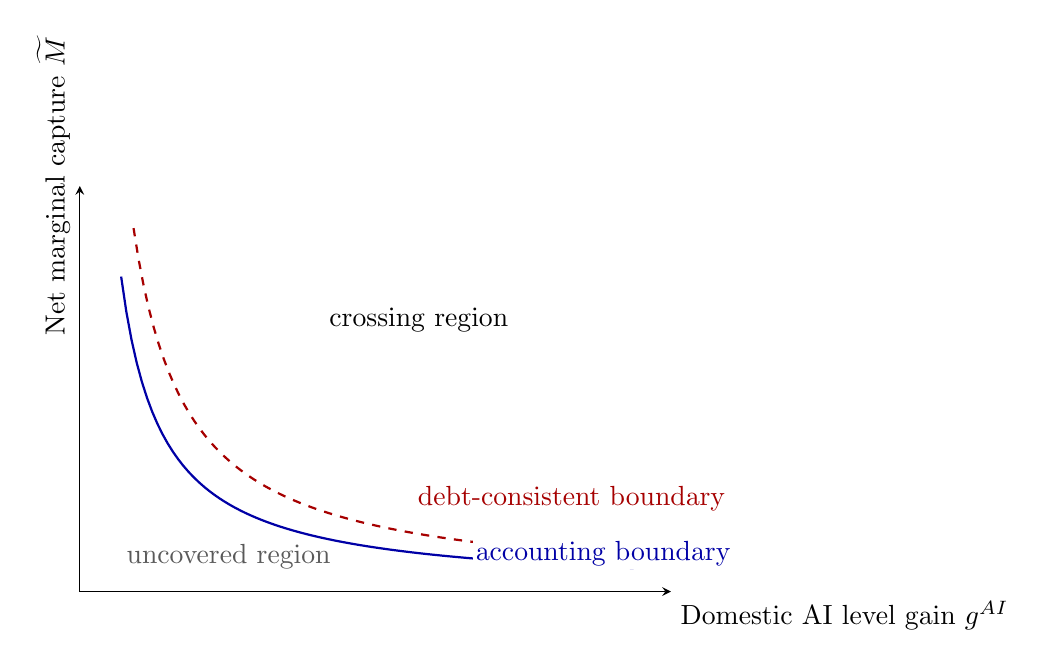
\begin{tikzpicture}[x=1.05cm,y=1.0cm,>=stealth]
  \draw[->] (0,0) -- (7.15,0)
    node[below right,align=center] {Domestic AI level gain $g^{AI}$};
  \draw[->] (0,0) -- (0,5.15)
    node[above left,rotate=90,anchor=south] {Net marginal capture $\widetilde M$};
  \draw[thick,blue!65!black,domain=0.5:6.7,samples=100]
    plot (\x,{2.0/\x});
  \draw[thick,dashed,red!65!black,domain=0.65:6.7,samples=100]
    plot (\x,{3.0/\x});
  \node[blue!65!black,anchor=west,fill=white,inner sep=1pt] at (4.75,0.48)
    {accounting boundary};
  \node[red!65!black,anchor=west,fill=white,inner sep=1pt] at (4.05,1.18)
    {debt-consistent boundary};
  \node[align=center] at (4.1,3.45) {crossing region};
  \node[align=center,text=gray!70!black] at (1.8,0.45) {uncovered region};
\end{tikzpicture}
\caption{Schematic feasibility boundaries. The solid curve satisfies
$\widetilde M g^{AI}=\mathcal R(\xi)$; combinations above it cross the buffered accounting threshold. The dashed curve adds the primary-balance correction, $\widetilde M g^{AI}=\mathcal R^{DC}(\xi)$. The axes are not drawn to empirical scale.}
\label{fig:frontier_clean}
\end{figure}

The same identities can be inverted to report requirements rather than a binary outcome. Suppressing indices and letting $\mathcal R$ denote either the accounting or debt-consistent requirement,
\begin{align}
  g^{AI,*}
    &=\frac{\mathcal R}{\widetilde{MFC}^{gross}},
  &MFC^{gross,*}
    &=\frac{\mathcal R}{g^{AI}}+D^{ME},
    \label{eq:g_mfc_inversions_clean}\\
  T^{req,H}
    &=\frac{\left(1+\mathcal R/\widetilde{MFC}^{gross}\right)^{1/H}-1}
            {\phi^{Y,nom}}.
    \label{eq:translation_inversion_clean}
\end{align}
These quantities answer how large the domestic gain, gross fiscal capture, or translation factor would have to be. The closed forms hold with channel weights fixed at the evaluated scenario, and the translation formula uses a constant annual scenario and domestic structure over $H$. Recomputing taxable-base composition as the shock changes, or allowing a time-varying path, turns the corresponding inversion into a numerical root. Appendix~\ref{app:derivations} provides the derivations. Since $T\leq1$, a requirement above one lies beyond the domestic-translation frontier. This diagnosis does not by itself make translation the sole constraint: several required margins can exceed their admissible or historically supported ranges at the same time.

The temporal inversion holds the scenario and domestic structure fixed and asks how long the annual translated increment would need to persist:
\begin{equation}
  H^*_{i,p,s,r}(\xi)
  =\min\left\{
    H\in\mathbb N:
    \widetilde{MFC}^{gross}_{i,s,r}
    \left[\left(1+\phi^{Y,nom}_{s}T_{i,s}\right)^H-1\right]
    \geq(1+\xi)c^{gross}_{i,p}(H)+F^{fix}_{i,p,s,r}
  \right\}.
  \label{eq:hstar_clean}
\end{equation}
The debt-consistent version adds $s_i^{PB}$ to the right-hand side. Endpoint costs may vary with the eligible population, which is why $c^{gross}(H)$ remains inside the definition. $H^*$ is a required persistence horizon, not a forecast date. It was introduced after the baseline as a derived reporting extension; it changes no calibrated input and no baseline classification.

Section~\ref{sec:design} maps these objects into country data, policy-cost rules, AI scenarios, fiscal regimes, and calibrated uncertainty.
